%!TEX root = practicum2.tex
The perceptron introduced by \citeauthor{rosenblatt1958perceptron} inspired many variations, one of those is the Minover algorithm by \citeauthor{krauth1987learning}. This algorithm aims to find the largest possible margin between two linearly separable classes. \Cref{fig:1:optimalSolution} illustrates the optimal separation between two classes according to the Minover algorithm and the area of all suboptimal separations that classify each available pattern correctly. 

\begin{figure}[H]
	\centering
	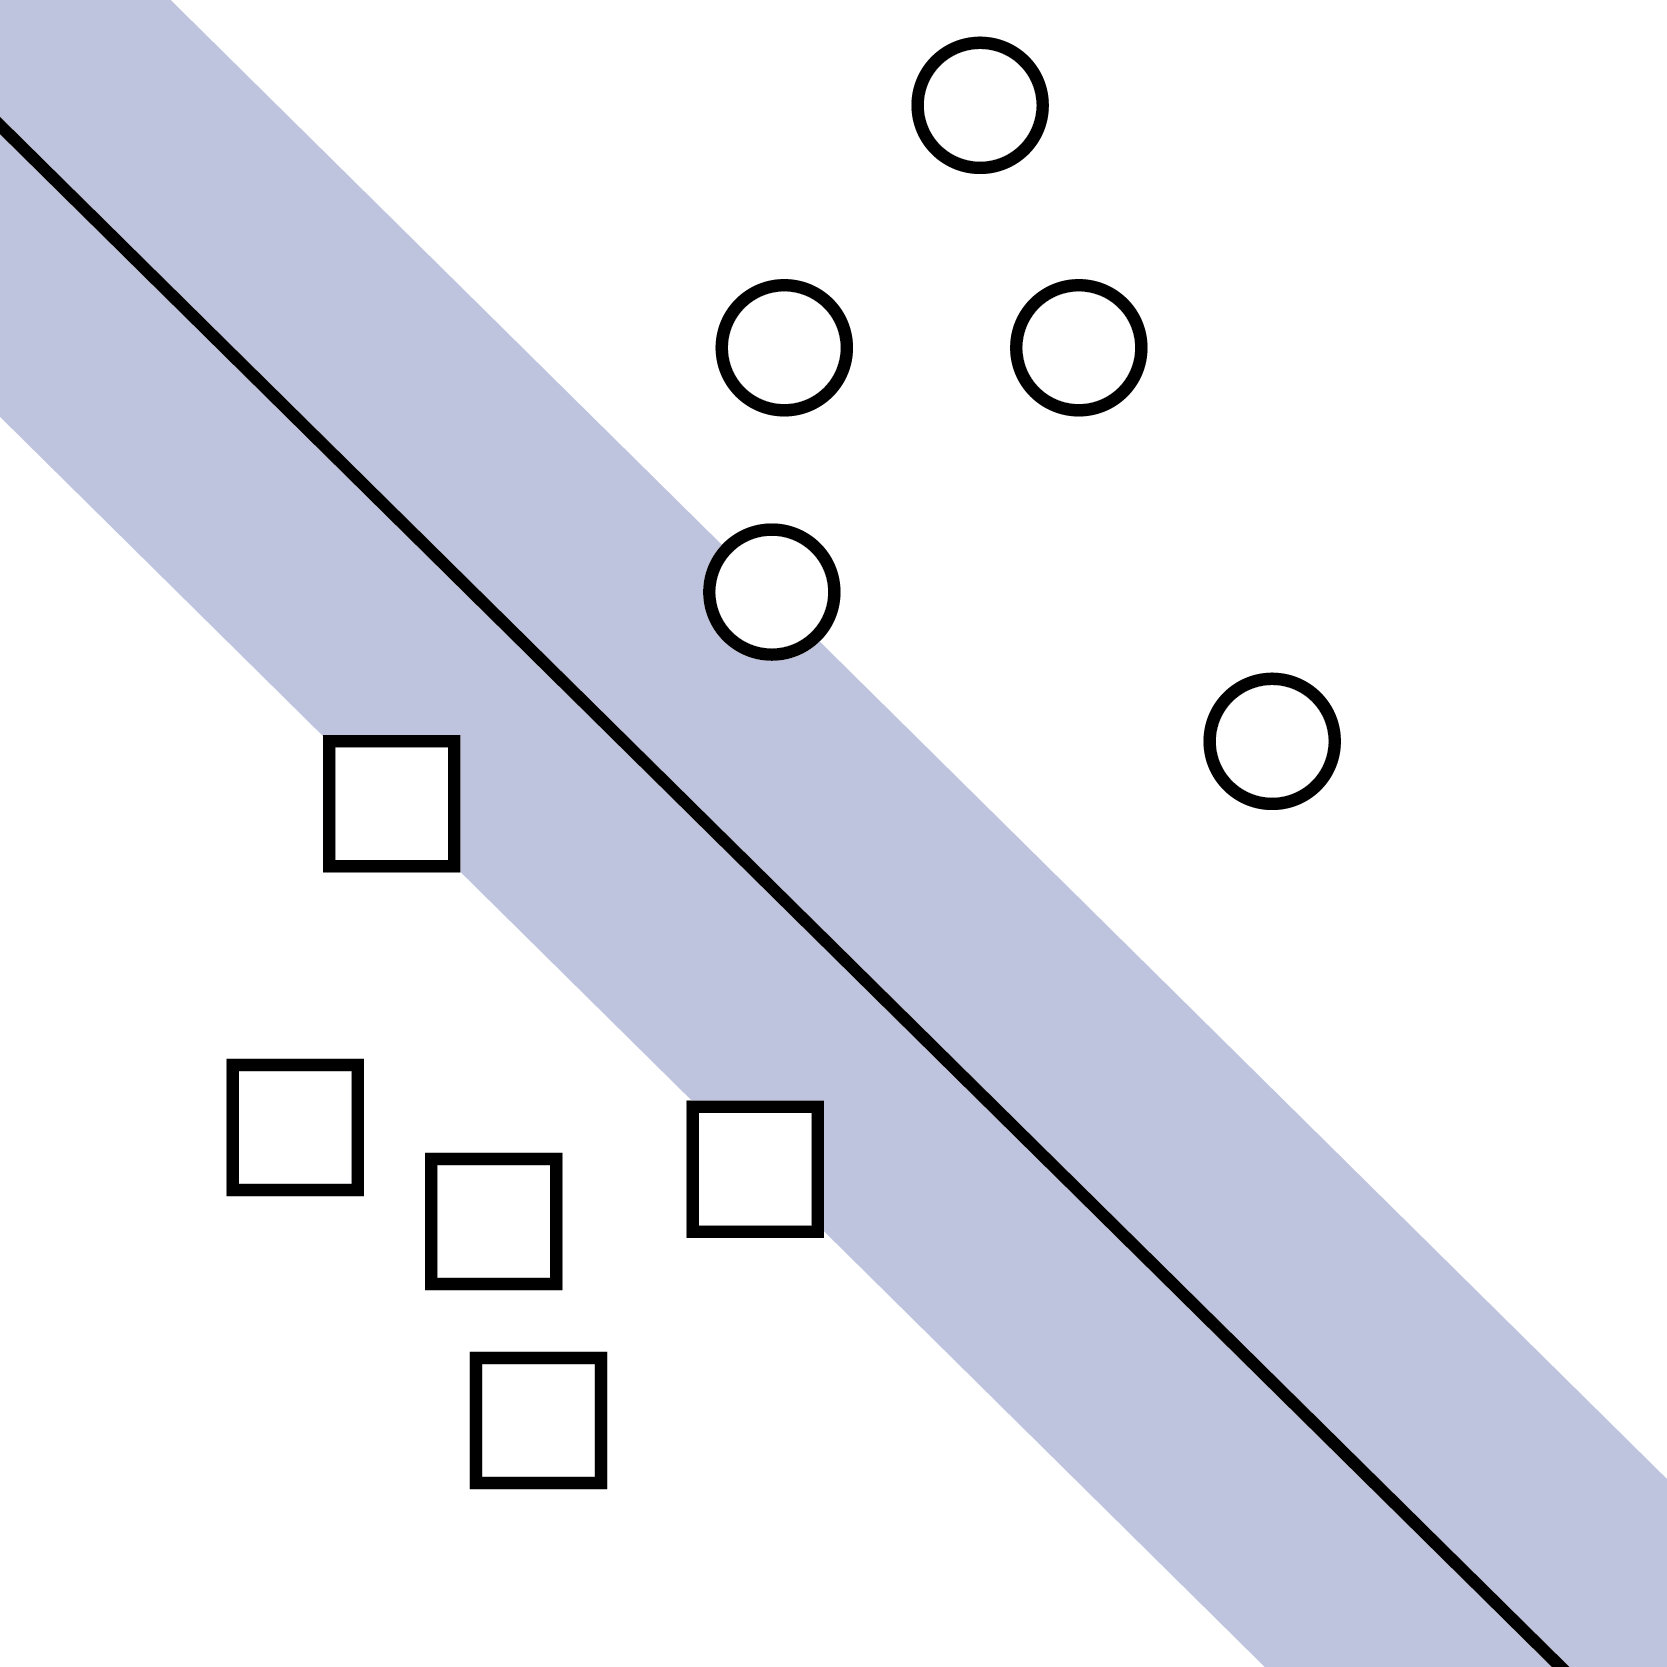
\includegraphics[width=0.9\columnwidth]{./img/optimalboundary-01}
	\caption{The separation of two classes, with the optimal boundary shown as the line. All suboptimal separations of the the two classes that separate the points correctly lie in the shaded area. The support vectors are indicated by the symbols with a border.}
	\label{fig:1:optimalSolution}
\end{figure}

\Cref{fig:1:optimalSolution} illustrates that the optimal boundary is determined by only three points, the support vectors, indicated by symbols with a border in \cref{fig:1:optimalSolution}. Changing the location of the other patterns does not influence the optimal decision boundary as long as they do not fall within the separation area.
